\section{Einleitung}
Das RoboCup-Projekt ist ein internationales Forschungs- und Bildungsprojekt. 
Ziel ist die Förderung der Erforschung künstlicher Intelligenz und 
Robotertechnik in einem konkreten Anwendungsumfeld: dem kooperativen 
Fußballspiel.
Dazu wird regelmäßig der \textbf{RoboCup} ausgetragen, eine Konferenz- und
Wettbewerbsveranstaltung, auf welcher diverse Wettkämpfe in verschiedenen Ligen
ausgetragen werden:

\begin{itemize}
  \item Simulationsliga (2D und neuerdings auch 3D)
  \item Small-Size-Liga
  \item Middle-Size-Liga
  \item Four-Legged-Liga
  \item Humanoid-Liga
  \item E-Liga
\end{itemize}

Mit dem RoboCupRescue-Projekt wird ein weiteres interessantes
Anwendungsfeld erschlossen: Die Suche und Rettung von Unfallopfern in unbekannten
Umgebungen durch kooperierende, mobile autonome Roboter.

\section{Das "`Mindstormers Tribots"' RoboCup-Team}
Ursprünglich entwickelt an der Universität Dortmund, ist das Team der 
"`Mindstormers Tribots"' heute am Institute of Cognitive Science an der 
Universität Osnabrück beherbergt. Neben einer Robotermannschaft der 
Middle-Size-Liga wird auch ein Simulationsteam betrieben. In den letzten Jahren 
konnten durch das Team diverse Wettbewerbserfolge erzielt werden, zuletzt 
erreichte das Middle-Size-Team im Jahr 2006 den Weltmeistertitel beim RoboCup 
in Bremen \cite{url:Neuroinformatics2006}.

In den folgenden Abschnitten werden die einzelnen Vorgehensweisen - 
insbesondere in Bezug auf das Training der Roboter - der Verantwortlichen 
sowohl in der Simulations- also auch in der Middle-Size-Liga vorgestellt.

\subsection{Simulationsliga (Brainstormers)}
In der Simulationsliga spielen zwei Teams mit jeweils elf virtuellen Agenten 
gegeneinander. Bei dieser Disziplin steht die Kooperation und Kommunikation 
unter den einzelnen Spieler-Instanzen besonders im Vordergrund. Zielsetzung ist 
die Übertragung der aus diesen Aspekten gewonnenen Erkenntnissen auf humanoide 
Roboter.
Um faire Wettbewerbsbedingungen zu garantieren, sind durch das entsprechende 
Komitee Regeln definiert, die sich im Prinzip an den FIFA-Fußballregeln 
orientieren.

\subsubsection{Funktionsweise der Simulation}
Die Simulation wird mittels einer Client-Server-Architektur realisiert. Der 
Server (offizielle Implementierung ist der \glq{}RoboCup Soccer Simulator\grq{} 
\footnote{\url{http://sserver.sourceforge.net}}) stellt dabei die Spielumgebung 
bereit und versorgt die einzelnen Clients mit (i.\,A.\ recht verrauschten) 
Sensorinformationen. Ein Client ist ein einzelner Spieler und wird durch einen 
separaten Prozess bzw.\ Thread realisiert. Clients können Aktionsbefehle an den 
Server senden und über diesen auch indirekt mit ihren Teammitgliedern 
kommunizieren.

Dies stellt bereits eine erste Einschränkung dar: Jegliche Kommunikation muss 
über den Server abgewickelt werden, wobei die Bandbreite des 
Kommunikationskanals beschränkt ist und somit nur ein sehr unvollständiger 
Informationsaustausch möglich ist.  Neben den Aktionsbefehlen (darunter z.\,B.\ 
\textsl{turn()}, \textsl{dash()} oder \textsl{kick()}) die der Server 
interpretiert, werden auch Umwelteinflüsse wie Reibung durch Boden und Wind 
sowie die Kondition der Spieler simuliert.
Die Simulation verläuft in Echtzeit - in einem Intervall von 100\,ms können die 
Clients eine Aktion durchführen und erhalten Sensorinformationen vom Server. 
Ein komplettes Spiel dauert 6000 Zyklen, was einer realen Zeit von 10\,Min. 
entspricht. Über eine sog.\ Monitor-Anwendung kann das Spielgeschehen 
visualisiert und live bzw.\ als Wiederholung verfolgt werden. Eine 
beispielhafte Spielszene ist in Abbildung \ref{fig:robocup-simulation-monitor} 
dargestellt.

\begin{figure}
  \centering
  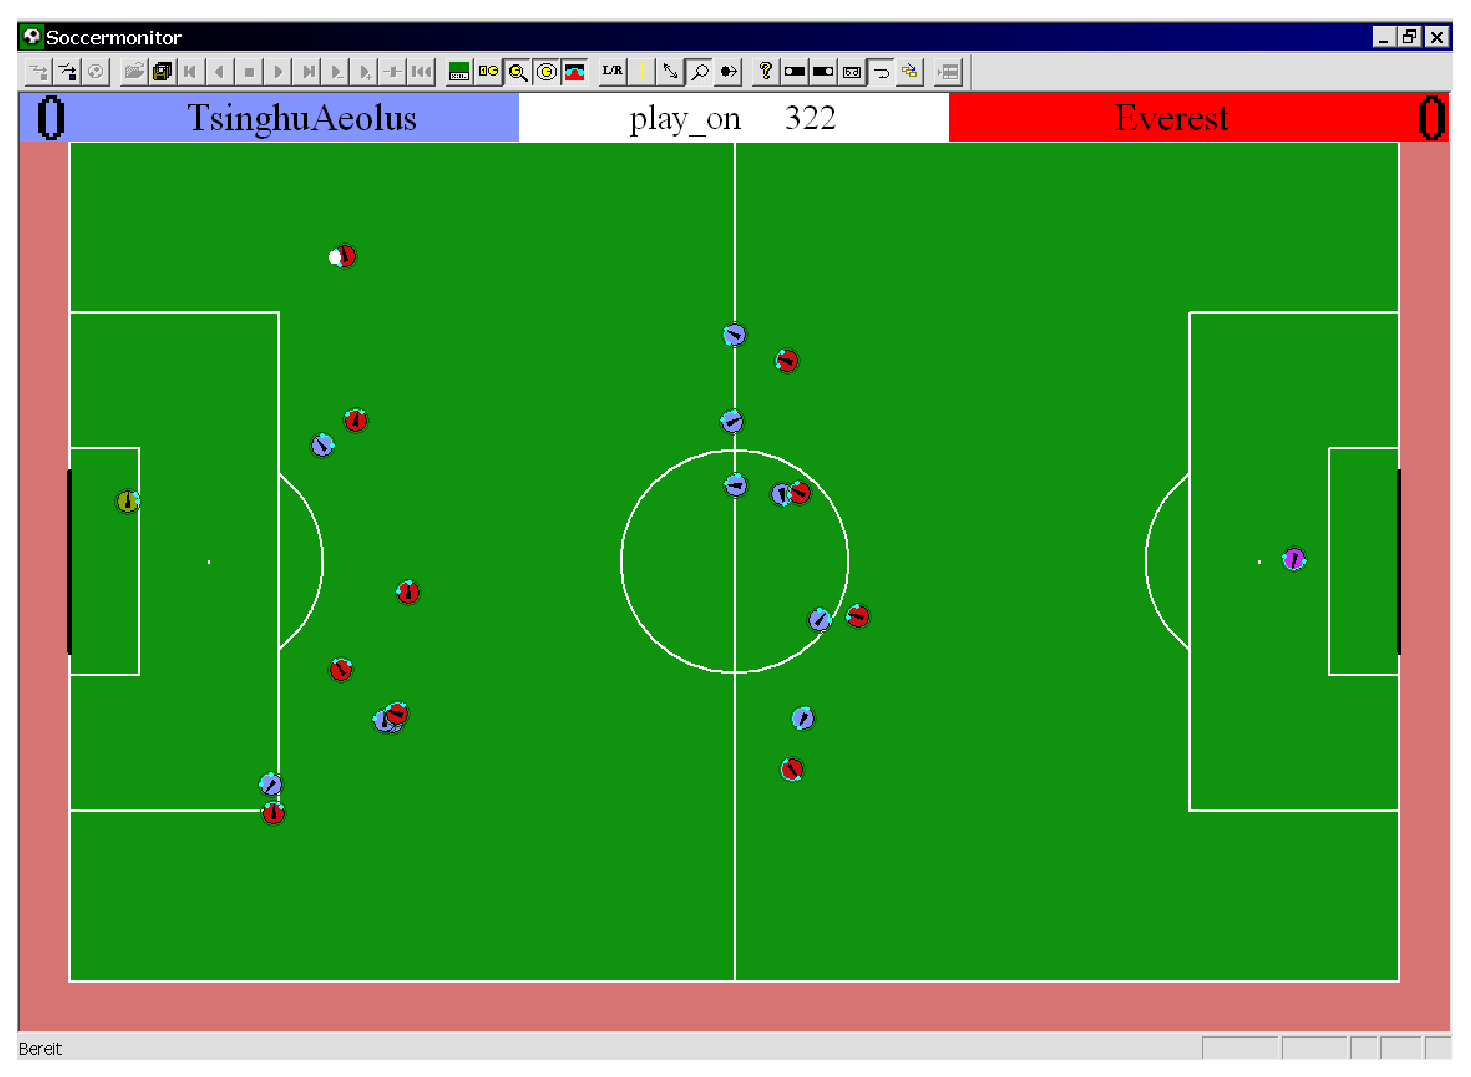
\includegraphics[width=0.80\textwidth]{../images/rcssmonitor_classic}
  \caption{RoboCup-Monitor: Visualisierung eines Spieles}
  \label{fig:robocup-simulation-monitor}
\end{figure}

Zusammenfassend ergeben sich bei der Simulation die folgenden Herausforderungen:

\begin{itemize}
  \item Aus den je 6000 Einzelentscheidungen eines jeden Spielers muss ein
  möglichst erfolgreiches, kooperatives Spiel entstehen.
  \item Sensorinformationen sind nur eingeschränkt und verrauscht verfügbar.
  \item Störungen bei Aktionsausführungen.
  \item Begrenzte Kondition der Spieler.
\end{itemize}

\subsubsection{Lernen von Einzelfähigkeiten}
Eines der allgemeinen Entwurfsprinzipien des Mindstormers-Teams ist die
Koexistenz und Austauschbarkeit von gelernten und ausprogrammierten
Verhaltensmodulen. Auf diese Weise können für einzelne Aufgaben jeweils 
verschiedenen Verfahren oder Strategien getestet und angewandt werden 
\cite{Riedmiller2006}.

Eine \textbf{Einzelfähigkeit} bezeichnet eine elementare technische Fähigkeit
eines einzelnen Spielers, die eine klar definierte Aufgabe zu erfüllen hat.
Beispiele dafür sind:

\begin{itemize}
  \item schnelles Abfangen eines rollenden Balles,
  \item effizientes Laufen zu einer Zielposition,
  \item Schießen des Balles mit spezifizierter Richtung und Geschwindigkeit,
  \item Ballhalten,
  \item Dribbeln.
\end{itemize}

Diese Einzelfähigkeiten werden aus sog.\ \textbf{Elementaraktionen} (z.B.
\textsl{dash()}, \textsl{turn()} oder \textsl{kick()}) zusammengefügt und
überführen den aktuellen Zustand in einen Zielzustand. Das Lernen einer
Einzelfähigkeit stellt nun ein dynamisches Optimierungsproblem dar, bei welchem
der Lernalgorithmus eine Strategie mit den minimalen Kosten für alle
Startzustände finden soll. Der Ablauf des Training stellt sich wie folgt dar:

\begin{enumerate}
  \item Auswahl einer Elementaraktion mit möglichst geringen Kosten.
  \item Bei Erreichen eines positiven Zielzustands: Ende der Lernsequenz
  \textsl{ohne} Kosten.
  \item Bei Erreichen eines negativen Zielzustands: Bestrafung durch hohe Kosten.
\end{enumerate}

Dieser Trainingsprozess erfolgt nun auf Episodenbasis. Ausgehend von einem
zufälligen Startzustand wählt der Spieler eine Elementaraktion - bei
Exploration eine zufällige, ansonsten diejenige mit den niedrigsten zu
erwartenden Kosten. Da das vom Server simulierte Umgebungsmodell bekannt ist,
kann der Spieler nun für alle Aktionen die Werte der Folgezustände berechnen,
was ihn befähigt, die für ihn günstigste Aktion auszuwählen. Wurde die Aktion
durchgeführt und die Kosten an den Spieler vergeben, wird die Wertfunkion
entsprechend aktualisiert.

\subsubsection{Lernen von Teamfähigkeiten}
Beim Lernen von Teamfähigkeiten ergibt sich das Problem, dass die Aktionsmenge
eines einzelnen Spielers exponentiell mit der Anzahl der Spieler anwächst,
außerdem steigt die Dimension des Zustandsvektors linear. Da aufgrund
dieser Probleme keine tatsächliche Teaminteraktion trainiert werden kann, führt
der Agent sog.\ Makroaktionen, also Kombinationen von zuvor gelernten
Einzelfähigkeiten, aus.

Um die Spieler zu einem kooperativen Spiel zu zwingen, erhalten sie alle 
dasselbe Reinforcement-Signal: das Erzielen eines Tors wird mit Nullkosten 
belohnt, das Verlieren des Balls mit Kosten von 1 bestraft. Tritt keines dieser 
beiden Ereignisse auf, so werden kleine konstante Kosten berechnet. Durch diese 
Modellierung geht jedoch nicht das Individualspiel eines einzelnen Spielers 
verloren, denn schließlich befindet sich jeder Spieler in einer anderen 
Situation und muss dementsprechend andere Aktionen ausführen. Die 
Entscheidungsfindung zur Auswahl einer Aktion läuft folgendermaßen ab:

\begin{enumerate}
  \item Alle Aktionen werden auf ihren möglichen Erfolg geprüft.
  \item Für alle erfolgreichen Aktionen wird über ein Modell der Folgezustand
  berechnet. Dieses Modell ist allerdings - aufgrund des unbekannten Mitspieler-
  und Gegnerverhaltens - nur approximativ. Es wird daher vereinfachend
  angenommen, dass gar keine anderen Spieler existieren.
  \item Der Folgezustand wird durch die Wertefunktion bewertet. Für diese
  Bewertung wird ein neuronales Netz mit 34 Eingängen, 10 verborgenen Neuronen
  und einem Ausgabeneuron eingesetzt (s.\ Abbildung \ref{fig:rl-neuronales-netz}).
  \item Die Aktion mit dem geringsten Wert wird durchgeführt.
\end{enumerate}

\begin{figure}
  \centering
  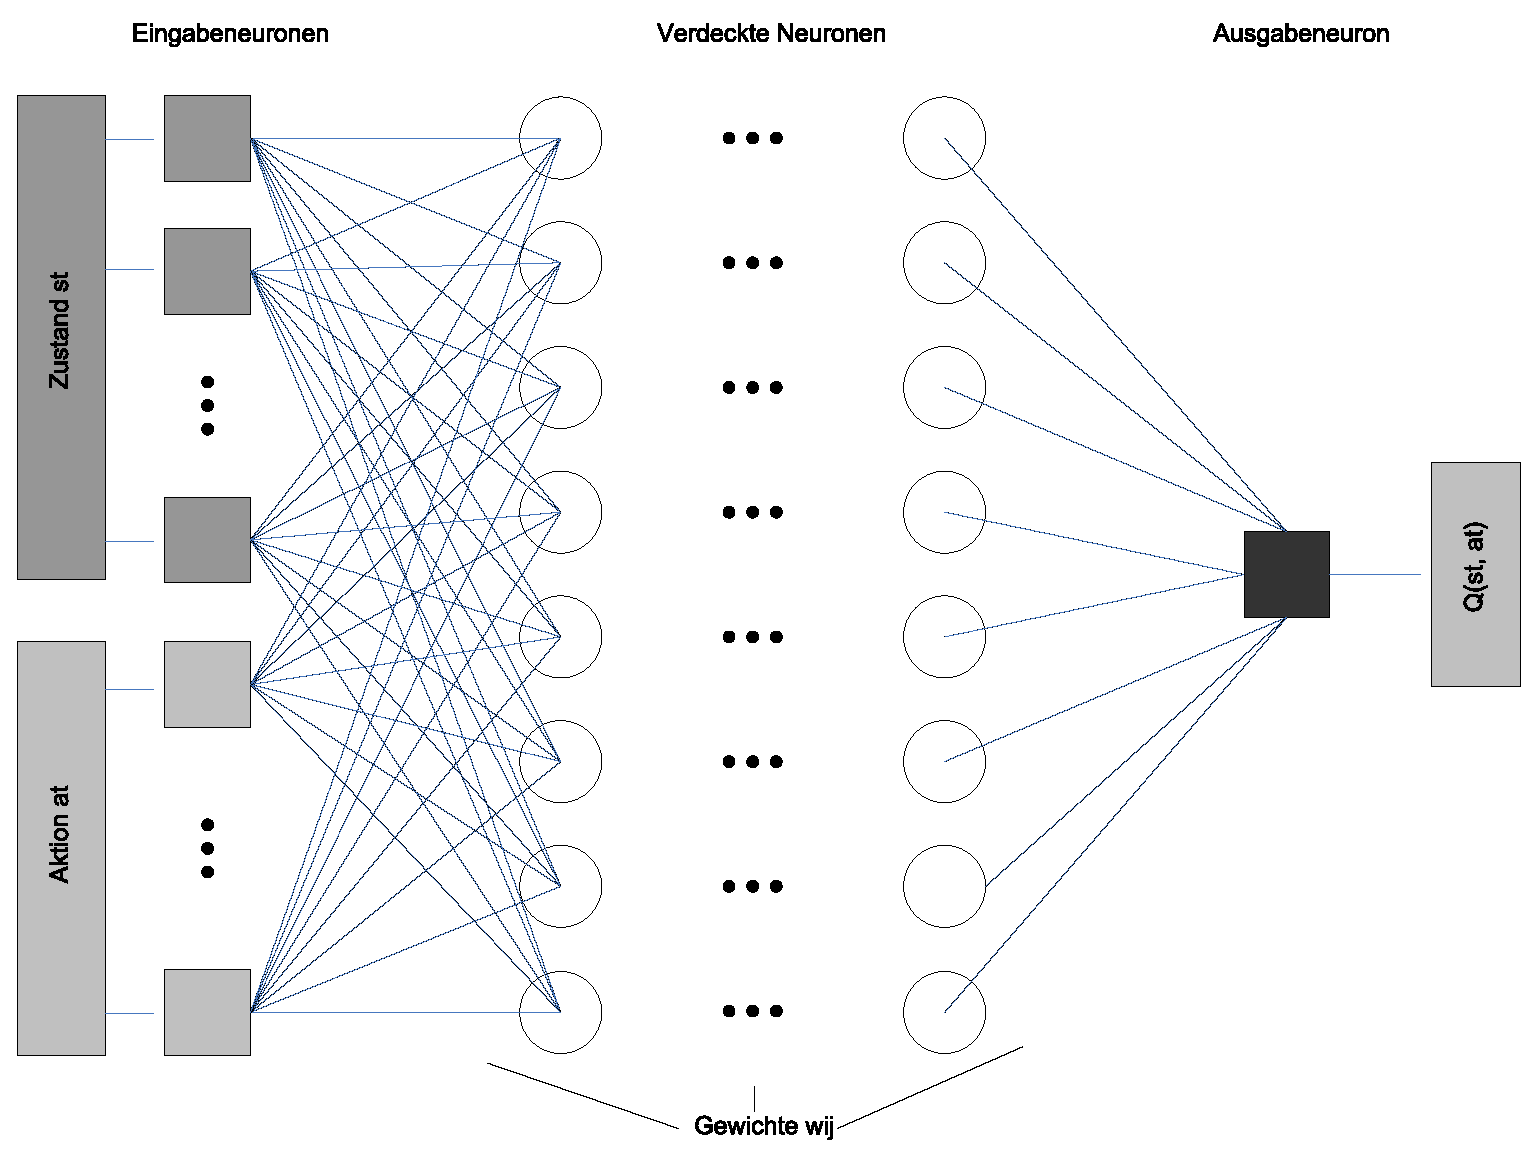
\includegraphics[width=1.00\textwidth]{../images/rl-neuronales-netz}
  \caption{Das eingesetzte neuronale Netz zur Approximation beim Q-Learning}
  \label{fig:rl-neuronales-netz}
\end{figure}

Während der Lernphase werden die gespielten Züge aufgezeichnet und anschließend
bzgl.\ der Kostenfunktion bewertet. Durch überwachtes Lernen kann das Netz diese
Bewertungen nun lernen und das neue Netz an die anderen Agenten verteilt werden.

\subsubsection{Fazit}
Es wurden die verschiedensten Fähigkeiten mittels des Reinforcement Learnings 
gelernt, die auch durchweg gute Spielleistungen erzielten. Allerdings konnten 
durch manuelle Optimierungen teilweise noch bessere Leistungen erzielt werden 
und so koexistieren im aktuellen Team sowohl manuell kodierte als auch erlernte 
Verhaltensmodule. Auffällig ist jedoch, dass im Jahr des Weltmeistertitels 
lediglich noch zwei erlernte Module im Einsatz waren - die restlichen erwiesen 
sich als nicht leistungsfähig genug.

\subsection{Middle-Size-Liga (Tribots)}
In der Middle-Size-Liga sollen allgemeine Anwendungsmethoden in der Robotik und 
der künstlichen Intelligenz wie z.\,B.\ Bildverarbeitung, Multi-Agenten-Systeme 
und Tra\-jek\-to\-ri\-en-Planung näher betrachtet werden.

Beim RoboCup-Wettbewerb treten in dieser Liga in der Regel vier mittelgroße 
Roboter, ausgestattet mit Onboard-Sensoren, auf einem Spielfeld der Größe 
12x8\,m gegeneinander an. Eine besondere Schwierigkeit stellt hier die 
durchzuführende Selbstlokalisation mittels der mitgeführten Kamera dar.

Die Roboter des "`Tribots"'-Team (s. Abbildung \ref{fig:tribots-roboter}) 
werden über ein dreirädriges Fahrwerk angetrieben und verfügen über ein 
omnidirektionales Kamerasystem sowie eine pneumatische Schusseinheit. Die 
Steuerung des Roboters wird über ein auf dem Chassis montiertes Sub-Notebook 
übernommen; die Kommunikation mit den anderen Teammitgliedern erfolgt über 
W-LAN \cite{url:Tribots2006}.

\begin{figure}
  \centering
  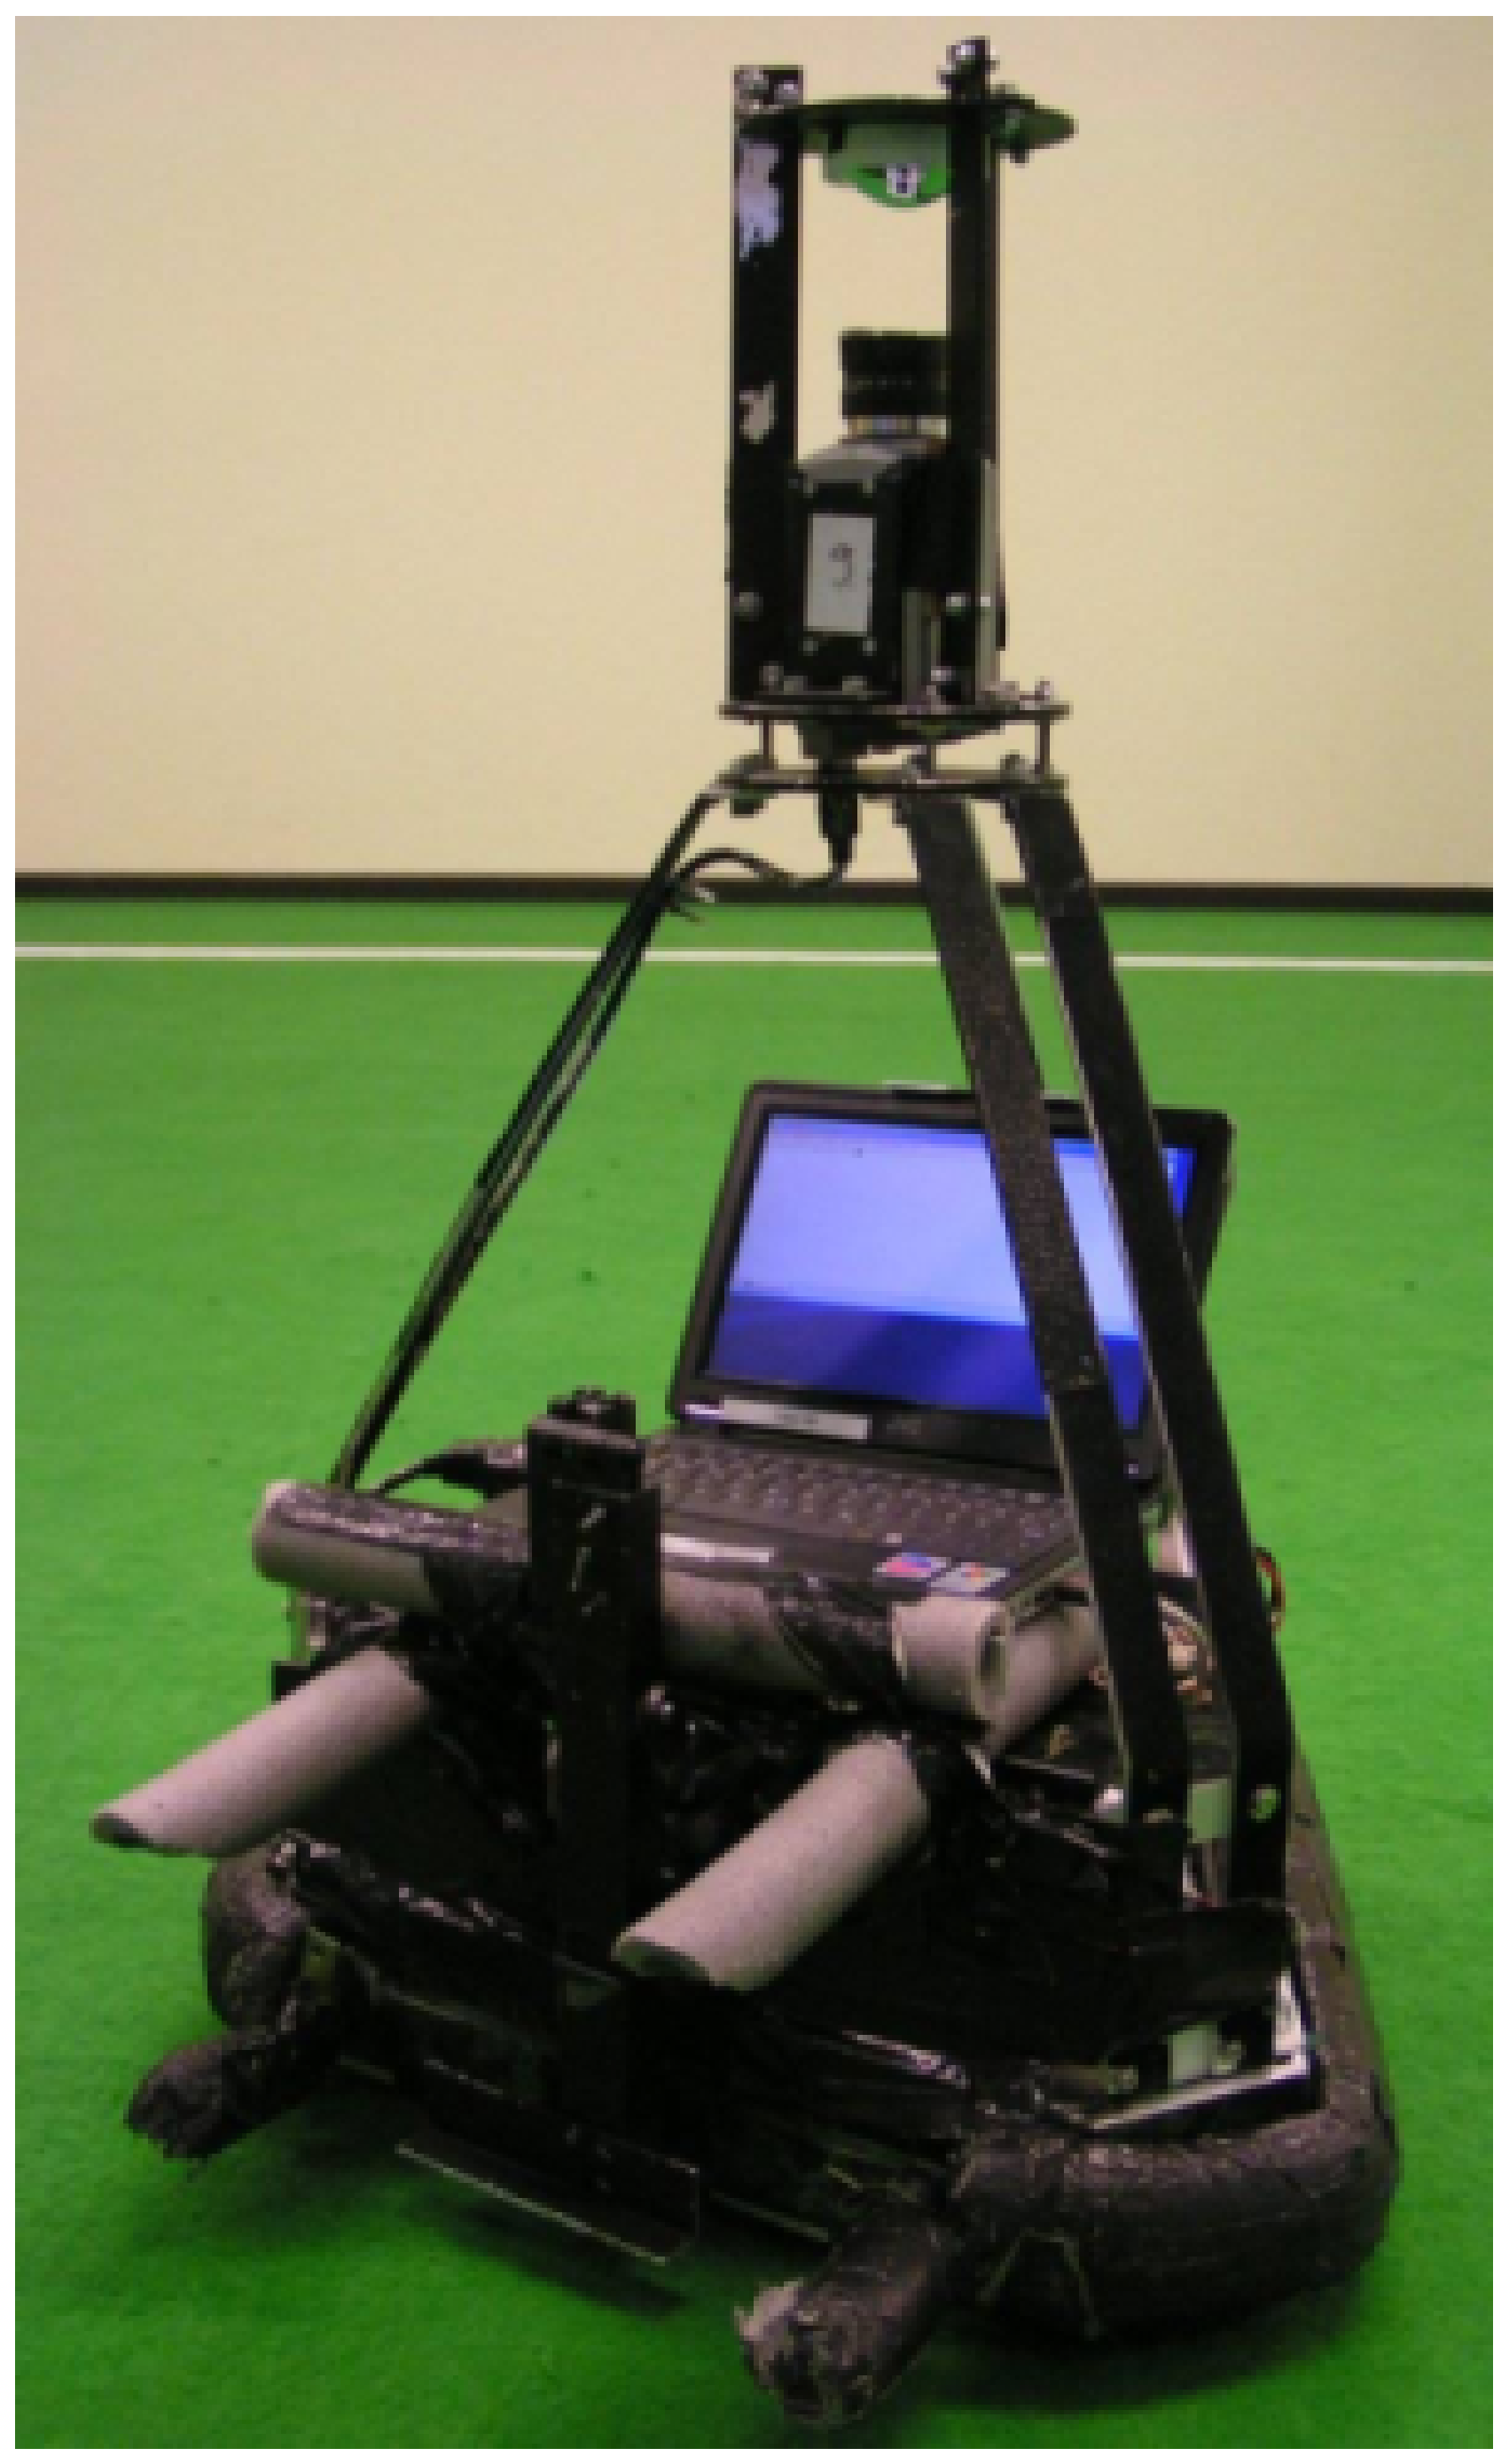
\includegraphics[width=0.40\textwidth]{../images/tribots-roboter}
  \caption{Ein Roboter des Tribots-Teams. Quelle: Webseite der Brainstormers Tribots}
  \label{fig:tribots-roboter}
\end{figure}

\subsubsection{Aufbereitung der Sensorinformationen}
Um dem Roboter ein möglichst genaues physikalisch-geometrisches Modell des 
aktuellen Spielgeschehens zur Verfügung zu stellen, werden zunächst über die 
Sensoren (omnidirektionale Kamera sowie Odometrie-Einheit) Daten der Umwelt 
gesammelt. Die zentale und wichtigste Information ist die eigene Position des 
Roboters auf dem Spielfeld. Diese wird über die von der Kamera aufgenommenen 
weißen Linien des Spielfelds bestimmt, zusätzlich werden die Daten des 
zurückgelegten Weges (Odometrie) benutzt. Allerdings sind diese beiden 
Sensorinformationen teilweise recht ungenau, weshalb kein tatsächlich exaktes 
Umweltbild ermittelt werden kann. Weiterhin muss die Ballposition und 
-geschwindigkeit sowie die Geschwindigkeit des Roboters ermittelt werden.

Ein Problem stellt die begrenzt zur Verfügung stehende Rechenkapazität dar. 
Dieser Umstand erfordert es, dass die Kamerabilder lediglich mittels eines sehr 
einfachen Farberkennungs- und Subsampling-Algorithmus verarbeitet werden, um so 
die verschiedenen Objekte anhand der Farben zuzuordnen: der Ball ist laut 
Regelwerk rot, die Tore blau und gelb sowie die Roboter schwarz. Neben der 
Erfassung des aktuellen Zustands wird außerdem über verschiedene Verfahren eine 
Vorhersage über zukünftige Parameter (also z.\,B.\ die Ballposition) getroffen.

Auf Basis des so erstellten Umweltmodells kann der Roboter nun das 
entsprechende Verhalten ausführen.

\subsubsection{Lernen von Einzelfähigkeiten}
Das Lernverfahren der Simulationsliga ist nicht direkt auf die realen Roboter 
anwendbar, da hier zu viele Lernversuche durchgeführt werden müssten. 
Stattdessen wählte man eine kombinierte Vorgehensweise: Der Lernvorgang wurde 
mit einem simulierten Roboter durchgeführt und diese Lerndaten anschließend auf 
den realen Roboter übertragen.
Am Beispiel des Verhaltens "`InterceptBall"' wird deutlich, dass die Lernaufgabe
tatsächlich nicht am realen Roboter hätte durchgeführt werden können. Denn das
mittels Q-Learning erlernte Verhalten benötigte 10 Mio. Iterationen, was einer
Realzeit von etwa 916 Std. entspräche.

Obwohl die so gelernten Verhalten auf dem realen Roboter die gewünschte Aktion
durchführen, bleibt das Problem, dass die optimale Eigenschaft durch die
Übertragung von Simulation auf Realität verloren geht. Aus diesem Grunde wurde
von den Verantwortlichen ein modifizierter Q-Learning-Algorithmus, die Neural
Fitted Q-Iteration, eingeführt. Dieses Verfahren erlaubt das Training direkt am
realen Roboter mit deutlich verringerter Interaktionszeit.

\subsubsection{Lernen von Regelungsaufgaben}
Von großer Bedeutung für einen mobilen Roboter ist die Fahrwerkssteuerung, da 
die erforderlichen Fahrtbewegungen (Richtung und Geschwindigkeit) möglichst 
präzise und schnell durchgeführt werden müssen.

Für die aktuelle Sollgeschwindigkeit wird für jeden einzelnen Motor eine 
separate Geschwindigkeit berechnet und der Motor entsprechend geregelt. 
Problematisch wird dies allerdings durch verschiedene Einflussfaktoren, wie 
z.\,B.\ die entstehende Reibung. Ausgehend von diesem Problem lässt sich das 
Verhalten des Geschwindigkeitsreglers auch mittels Reinforcement Learning 
lernen und somit optimieren.

\subsection{Fazit}
Die Erfahrungen mit Reinforcement Learning des Osnabrücker RoboCup-Teams waren 
i.\,A.\ positiv und die Qualität der gelernten Module überstieg anfangs jeweils 
die des handcodierten Pendants. Durch die gewonnenen Erkenntnisse beim Einsatz 
des Verstärkungslernens konnten einige der Module daraufhin optimiert werden, 
sodass letztlich doch eine handcodierte, minimal leistungsfähigere Variante in 
den Wettkämpfen zum Einsatz kommt.

Gerade diese Rückkopplung und die Kombination klassischer und erlernter Module 
werden als zukunftsfähig angesehen, u.\,a.\ in industriellen Anwendungen wie 
der Regelungstechnik oder reaktivem Scheduling.